\section{Introduction}
\label{sec:introduction}
Recent studies show that variable-length text types are among the most commonly used column data types in \acp{DBMS}.
For example, van Renen et al~\cite{van_renen_why_2024} showed that 52.1\% of all columns in the
Amazon Redshift are of this type.
But already in 2018, Vogelsgesang et al.~\cite{vogelsgesang_get_2018} showed with their analysis of Public Tableau
Workbooks that 48.8\% of their columns are of type text.
Most interestingly, these columns not only occur frequently but are also commonly used in operators and expressions.
For example, a workload analysis of the Snowflake Data Cloud performed by Szlang et al.~\cite{szlang_workload_2025}
shows that 46\% of join keys, 58\% of filter columns are text columns.
The reason why strings are so prevalent is that they are a catch-all type for many
different kinds of data and allow a very pragmatic schema design.
However, this often results in data being stored in formats that are inefficient for processing~\cite{vogelsgesang_get_2018}.

This prevalence of variable-length text columns poses significant challenges for query processing and storage management.
Unlike fixed-length numeric or boolean types, strings require dynamic memory allocation, incur higher CPU costs during
standard operations like comparison and hashing.

In this paper, we analyze how variable-length text columns are used in \acp{DBMS} and how they affect system performance
in execution and compression.
We argue that, to adequately address the heterogeneity of the data these columns can represent, it is necessary to
classify strings according to their semantic type.
Doing this, we create a \textit{taxonomy of variable-length text columns} by using \acp{LLM} to categorize string
columns as Numeric, Categorical, FullText, Identifier, Entity, or Semistructured.
Doing this, we show that which each of these classes we can see distinct physical characteristics
(length, character distribution) and usage patterns in query execution that can be exploited for efficient query processing.

As a data basis for this analysis, we use queries, schema information, and data from publicly available repositories.
Our work differs from previous studies such as~\cite{van_renen_why_2024, vogelsgesang_get_2018, szlang_workload_2025}
in that we also release a dataset containing detailed information about the analyzed tables, columns, queries,
query execution traces, column usages, and compression results.

In summary, we offer the following contributions:
\begin{itemize}
    \item We release a public dataset of real-world schemas, queries, and query plans.
    \item We present a reproducible pipeline for dataset creation.
    \item We propose a taxonomy for variable-length text columns and analyze their physical properties, usage patterns, and compressibility.
    \item We examine variable-length text column usage in the TPC-[H, DS] and SqlStorm benchmarks.
    \item Based on our findings, we provide recommendations for future research directions.
\end{itemize}

\section{Dataset Collection}\label{sec:data-collection}

To analyze the usage of text columns in \ac{DBMS}, we require both queries and corresponding populated tables.

One publicly available dataset that offers this is SchemaPile~\cite{dohmen_schemapile_2024}, which is a collection of database schemas extracted from DDL and DML statements found in SQL files across public code repositories.
However, as SchemaPile only contains data from SQL table dumps instead of database files or csv/parquet files.
This leads to a table only containing 27.6 values on average.
Since SchemaPile only provides schema and table information but no \texttt{SELECT} statements, we revisited the corresponding repositories to scrape such statements.
This process and resulting dataset characteristics are described in \cref{subsec:sqlpile-dataset}.

To complement the data with information on larger tables, we additionally analyzed data found publicly on kaggle.
These datasets are mostly designed for analytical workloads and contain both the data and the schema; however, they rarely include queries.
More information on this can be found in \cref{subsec:kaggle-datasets}.

Additionally, we analyzed the data and queries from both TPC-H, TPC-DS, and SQLStorm to identify further string usage patterns and to compare these benchmarks against the other datasets.

\subsection{SQLPile Dataset}\label{subsec:sqlpile-dataset}

In order to analyze the string usage in the scraped repositories, we first create and populate the tables featured in the
repository to then execute the select queries.
We decided to use DuckDB~\cite{raasveldt_duckdb_2019} as the database system, as it is fast
and easy to set up locally.

In total, we retrieved 36,991,829 queries from 27,389 repositories,
with 752,655 \texttt{SELECT}. By parsing the \texttt{CREATE} SQL statements, we could extract
701,382 distinct tables with 4,794,784 columns. In order to execute the queries
later in DuckDB, we unified the system specific column types into abstract types like \texttt{INTEGER}, \texttt{FLOAT}, 
\texttt{TEXT} or \texttt{DATETIME} to then later map them to the DuckDB types. 

For each repository, we then created a DuckDB database and created the tables using the parsed \texttt{CREATE} statements.
We then executed all the \texttt{INSERT} statements to populate the tables with data. Due to errors in the extracted 
SQL and differences in the features, data types and SQL dialects across systems, we could only execute 86.33\% 
of the \texttt{CREATE TABLE}, 83.83\% of the \texttt{CREATE VIEW} and 93.76\% of the \texttt{INSERT} statements. 
From this, we could populate 6,407 tables with at least one row, 
with a median of 5 rows and a mean of 100.59 rows per table.

To analyze string usage in the examined repositories, we executed the scraped \texttt{SELECT} statements.
Since queries are rarely written as static strings in the code, we first had to preprocess them by 
replacing variables and applying minor transformations to make them executable in DuckDB. This way, we where 
able to execute 27.59\% of the \texttt{SELECT} statements resulting in a 
total number of 56,222 statements we could retrieve query plans for. 

To then be able to track the usage of columns through the operators, we implemented a special 
explain function\footnote{See \url{https://todo}} that returns not only information on 
the operators used to execute the queries but also the details on the expressions these use. 

\begin{itemize}
    \item We also added SQLStorm and TPC-[H, DS] as benchmarks to compare against
\end{itemize}

\subsection{Kaggle Dataset}\label{subsec:kaggle-datasets}

\begin{itemize}
    \item How many datasets, tables, rows, columns
\end{itemize}


\section{Semantic Type}\label{sec:semantic-type}

Strings are a catch-all storage type; their semantics depend on how they are used.
To recover those semantics, we used an instruction-following LLM (Qwen3.5 via Ollama, \texttt{qwen3:8b}) with structured output to assign a single semantic label to every string-typed column.
For each candidate column we collected up to ten \emph{distinct, non-empty} sample values.
To keep the prompt compact and comparable across columns, the concatenated examples per column were truncated to a maximum length of \(\leq 100\) characters. Columns were processed in mini-batches of \(B=5\) to amortize model overhead while keeping responses aligned.

\subsection{Semantic Type Pipeline}\label{sec:semantic-type-pipeline}

We use and report twelve semantic types in total which are listed in \cref{tab:semantic-types-list}
along with the description we provided to the model.

\begin{table}
\caption{Semantic types for string columns and their model descriptions.}
\label{tab:semantic-types-list}
\begin{tabular}{lp{0.32\textwidth}}
\toprule
\textbf{Type} & \textbf{Type Description} \\
\midrule
\texttt{Name}           & Names of entities and persons, titles, labels \\
\texttt{DateTime}       & Dates, timestamps, time-related columns  \\
\texttt{Numeric}        & E.g.\ amounts, counts, prices, scores, sizes  \\
\texttt{Boolean}        & Yes/no flags, is*/has*, enabled states \\
\texttt{Category}       & Type, role, status, label, class, tag \\
\texttt{FullText}       & Descriptions, messages, summaries, notes, comments \\
\texttt{Identifier}     & Id, uuid, code, hash, token, version \\
\texttt{Contact}        & Emails, phone, fax, mobile \\
\texttt{Location}       & City, country, region, address, zip  \\
\texttt{URL}             & Link, url, image path, icon, slug \\
\texttt{Semistructured} & Formats like \texttt{JSON}, \texttt{CSV}, or simple lists \\
\texttt{Test}           & Column with content or name that are for testing (e.g., \texttt{test}, \texttt{col}, \texttt{val1}). \\
\bottomrule
\end{tabular}
\end{table}

We have one system message that is used for all batches:
\begin{quote}
    \small
    \texttt{Based on the table name, column name, and sample values, determine the semantic type of each column.
    Every column must fit one of the types:}\\
    \texttt{<type\_1>} \texttt{<type\_1\_description>}\\
    \(\dots\)\\
    \texttt{<type\_N>} \texttt{<type\_N\_description>}\\
    \texttt{You will be given multiple columns at once.
    Return *only* the list of semantic types in the same order as the columns were provided.}
\end{quote}

Each batch is rendered into a single user message of the form:
\begin{quote}
    \small
    \texttt{Determine the semantic type for each of the following columns:}\\
    \texttt{Column 1:}\\
    \texttt{Table: <table\_name>}\\
    \texttt{Column: <column\_name>}\\
    \texttt{Sample Values: [v\_1,\dots,v\_k]}\\
    \(\dots\)\\
    \texttt{Column N: \dots}
\end{quote}
\caption{Semantic types used for string columns and their intended interpretation.}
\label{tab:semantic-types}

Here should then come a detailed analysis in form of a table e.g. that shows example values for each operator and semantic
type e.g. how do the string columns look like. Also, for each semantic type, I would like to show what expressions where used.
For example, if there is a group by on a full text column, the query could look like
GROUP BY full\_text\_column LIKE 'foo\%' is probably not that useful.
\begin{itemize}
    \item
\end{itemize}

\subsection{Results}\label{sec:semantic-type-results}
%    \input{content/gen/sec_semantic_type_results}


\section{Storage}\label{sec:storage}

In this section, we want to analyze how much storage is used for different logical types and semantic types.

\begin{figure}
  \centering
  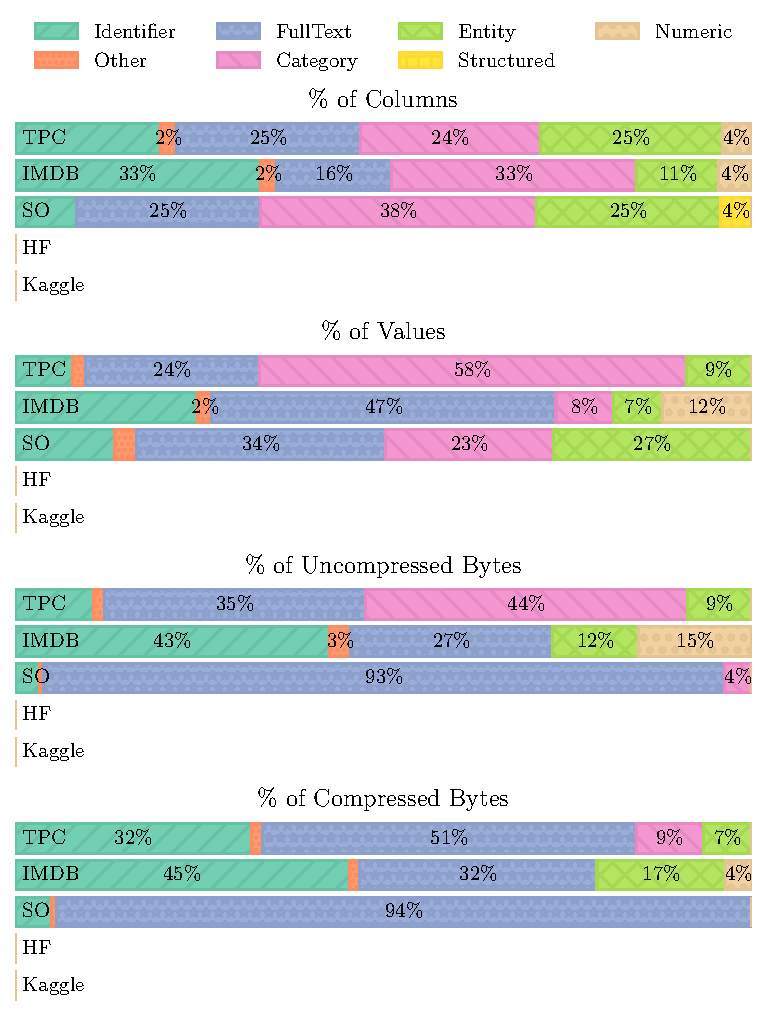
\includegraphics[width=\linewidth]{assets/semantic_type_llm.pdf}
  \caption{Ratios for storage for all strings based on semantic type}
  \Description{fig:storage-column-base-type}
  \label{fig:storage-column-base-type}
\end{figure}

\begin{figure}
  \centering
  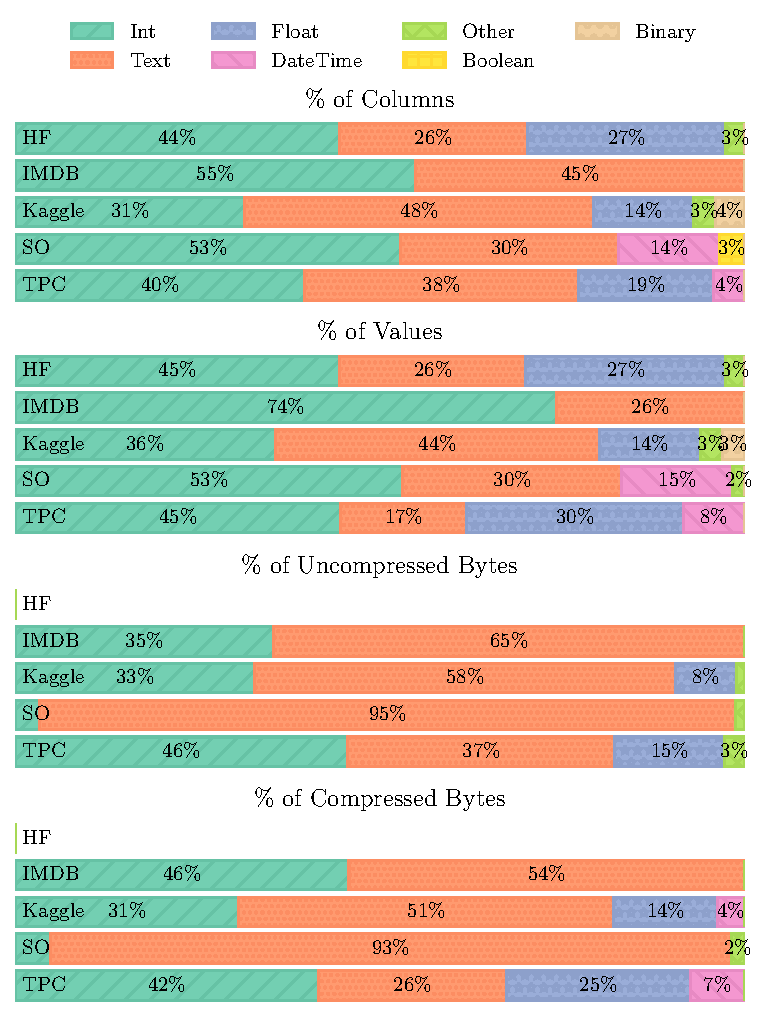
\includegraphics[width=\linewidth]{assets/column_base_type.pdf}
  \caption{Analysis on the storage per logical types}
  \Description{fig:storage-semantic-type-llm}
  \label{fig:storage-semantic-type-llm}
\end{figure}



\section{Properties of Strings}

As stated in our introduction, we aim to answer how different groups in our string taxonomy differ in their 
characteristics (RQ2).
Therefore we analyzed string columns from Kaggle, Huggingface, IMDB and Stackoverflow.
For each column, we compute the count, null count, empty count, distinct count, length percentiles, a value histogram, a char histogram
and more, which is available in DBPile's \texttt{column\_stats\_text} table.

In DBMS storage engines and analytical file formats such as Parquet \cite{NEEDED}, values are stored
and compressed in row groups of a fixed size.
All statistics in this work are computed at the level of a single row group.
For this paper, we assume a row group size of 122,880 values, which corresponds to the default configuration used by DuckDB.
As these statistics also correlate with compressibility, we want to have the same methodology in retrieving the column stats as the compression results.

\begin{figure}[h!]
  \centering
\begin{subfigure}{0.35\linewidth}
   \centering
  
\includegraphics[width=\linewidth]{assets/string_stats/duplicates/TPC/All_duplicates.pdf}
  \caption{TPC-[H/DS]}
  \label{fig:string_properties_dups_tpc_vs_others:all_duplicates}
\end{subfigure}
\begin{subfigure}{0.35\linewidth}
   \centering
  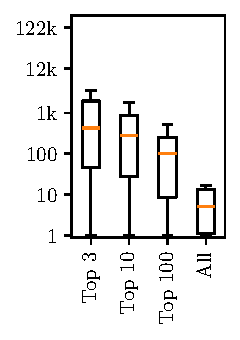
\includegraphics[width=\linewidth]{assets/string_stats/duplicates/Other/All_duplicates.pdf}
  \caption{Other}
  \label{fig:string_properties_dups_tpc_vs_others:all_duplicates}
\end{subfigure}
  \label{fig:string_properties_dups_tpc_vs_others}
  \caption{Duplicate value rates for TPC-[H/DS] datasets vs. all other datasets.}
\end{figure}

First, we examine how many duplicates string columns contain and how these duplicates are distributed. 
For this, we only considered columns with at least 122{,}880 values. Duplicate empty or null values 
do not count as duplicates. We omitted columns from the TPC schema, as they are known to follow a 
uniform distribution that does not reflect real-world data~\cite{NEEDED}. This also applies to TPC string 
columns, as shown in \cref{fig:string_properties_dups_tpc_vs_others}.

The figure shows that real-world datasets have both a more skewed value distribution and fewer duplicates on 
average than TPC columns. This aligns with our taxonomy results: 33\% of TPC columns are categorical, 
compared to an average of 20\%, and categorical columns naturally exhibit more duplicates.

Todo: cite https://link.springer.com/chapter/10.1007/978-3-642-32627-1_10 (Skewed TPC)

\insight{Strings in real-world datasets contain less duplicates but are more skewed than those in TPC datasets.}

\begin{figure*}[h!]
  \centering
\begin{subfigure}{0.1583\linewidth}
   \centering
  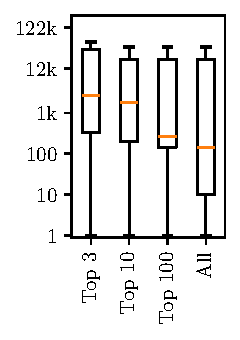
\includegraphics[width=\linewidth]{assets/string_stats/duplicates/Other/Category_duplicates.pdf}
  \caption{Category}
  \label{fig:string_properties_dups:category_duplicates}
\end{subfigure}
\begin{subfigure}{0.1583\linewidth}
   \centering
  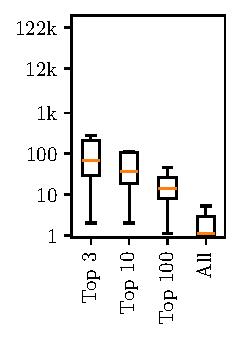
\includegraphics[width=\linewidth]{assets/string_stats/duplicates/Other/Entity_duplicates.pdf}
  \caption{Entity}
  \label{fig:string_properties_dups:entity_duplicates}
\end{subfigure}
\begin{subfigure}{0.1583\linewidth}
   \centering
  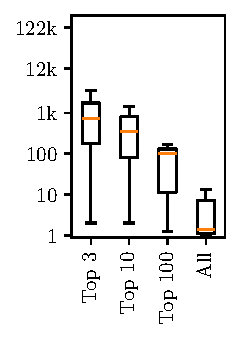
\includegraphics[width=\linewidth]{assets/string_stats/duplicates/Other/FullText_duplicates.pdf}
  \caption{FullText}
  \label{fig:string_properties_dups:fulltext_duplicates}
\end{subfigure}
\begin{subfigure}{0.1583\linewidth}
   \centering
  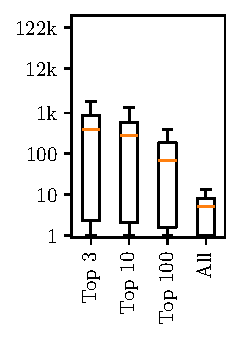
\includegraphics[width=\linewidth]{assets/string_stats/duplicates/Other/Identifier_duplicates.pdf}
  \caption{Identifier}
  \label{fig:string_properties_dups:identifier_duplicates}
\end{subfigure}
\begin{subfigure}{0.1583\linewidth}
   \centering
  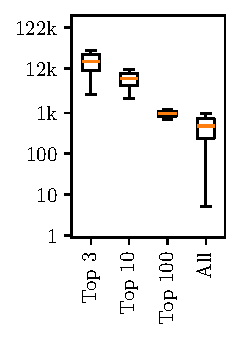
\includegraphics[width=\linewidth]{assets/string_stats/duplicates/Other/Numeric_duplicates.pdf}
  \caption{Numeric}
  \label{fig:string_properties_dups:numeric_duplicates}
\end{subfigure}
\begin{subfigure}{0.1583\linewidth}
   \centering
  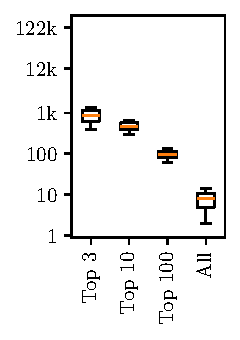
\includegraphics[width=\linewidth]{assets/string_stats/duplicates/Other/Structured_duplicates.pdf}
  \caption{Structured}
  \label{fig:string_properties_dups:structured_duplicates}
\end{subfigure}
  \label{fig:string_properties_dups}
  \caption{Duplicates per row group (122,880 values) per semantic types for all columns excluding TPC-[H/DS] datasets. Only strings that are not null or empty are considered.}
\end{figure*}

That categorical values contain many duplicates is also confirmed by \cref{fig:string_properties_dups}, 
which shows the number of duplicates for different groups in our taxonomy. The figure shows duplicates 
per row group of 122{,}880 for the top 3, 10, and 100 most frequent values, compared to the duplicates across all values.

Categorical columns have the highest duplicate ratios, with a median of 6 duplicates. 
Unlike the other groups, categorical columns show similar duplicate counts for the top 10 and top 100 values. 
This is because they have on average only 12864 distinct values, meaning that the top 10
already includes nearly all values for most columns.

Groups in which a substantial share of columns contain no duplicates include FullText and Identifier columns,
 and to some extent Entities. However, all of these groups still show notable amounts of duplication overall. 
 For Entities, this is expected, since values such as names come from a finite domain. For Identifiers, duplicates 
 can arise from foreign key relationships. For FullText columns, however, duplication is unexpected. Further 
 analysis shows that duplicates in FullText columns occur mainly in Kaggle and Huggingface datasets used for ML 
 applications.

\begin{figure*}[h!]
  \centering
\begin{subfigure}{0.15\linewidth}
   \centering
  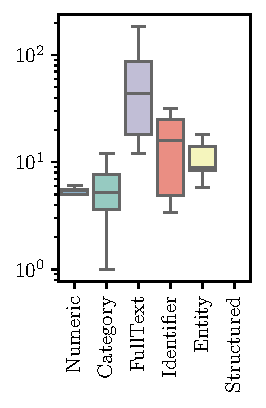
\includegraphics[width=\linewidth]{assets/string_stats/avg_length.pdf}
  \caption{avg. length}
  \label{fig:string_properties:avg_length}
\end{subfigure}
\begin{subfigure}{0.15\linewidth}
   \centering
  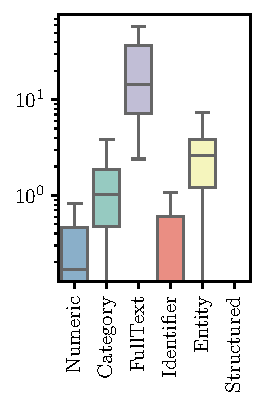
\includegraphics[width=\linewidth]{assets/string_stats/stddev_length.pdf}
  \caption{std. dev. length}
  \label{fig:string_properties:stddev_length}
\end{subfigure}
\begin{subfigure}{0.15\linewidth}
   \centering
  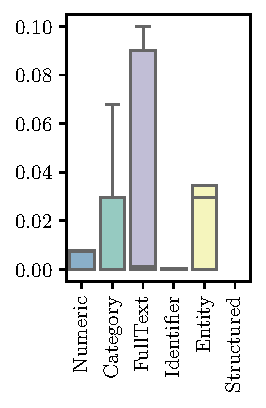
\includegraphics[width=\linewidth]{assets/string_stats/empty_or_null_rate.pdf}
  \caption{\% null or empty }
  \label{fig:string_properties:empty_or_null_rate}
\end{subfigure}
\begin{subfigure}{0.15\linewidth}
   \centering
  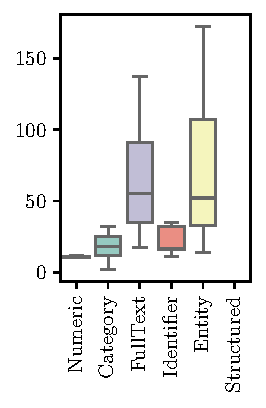
\includegraphics[width=\linewidth]{assets/string_stats/count_unfiltered.pdf}
  \caption{\# distinct chars}
  \label{fig:string_properties:count_unfiltered}
\end{subfigure}
  \label{fig:string_properties}
  \caption{String properties per semantic type for columns with at least 10,000 rows (n=330).}
\end{figure*}

In \cref{fig:string_properties}, we analyze the length and character distribution of different groups in our taxonomy.
We can see that the length of a string varies significantly between groups. FullText columns have the highest lengths,
and also the standard deviation of lengths. Categorical columns, on the other hand, have are often short, 
with 0.0\% having only one character, representing flags or codes. 

Identifier columns are longer, with a average length of 17.2 characters.
However, the standard deviation of lengths for Identifiers is relatively low, with 
41.2\% of columns having all identifier values of the same length. 
The reason for this is mainly uuid identifiers with the top three most common fixed-lengths being 32 (86\%) and 36 (14\%). 
Note that this exceeds both the 12 inline bytes permitted for German strings~\cite{neumann_umbra_2020} and the 16 
bytes that a \texttt{compact\_str}~\cite{timmerman_parkmycarcompact_str_2025} like implementation would inline. 
This also suggests execution-level opportunities: for instance, hashing logic for variable-length 
strings could employ a specialized fast path for these fixed-length identifiers. This shows that there is optimization
potential, such as a specialized hashing path for fixed-length identifiers stored as variable-length strings.

\insight{Different groups in our taxonomy exhibit distinct properties. E.g. identifiers are often 
uniform in length, categorical values are often short, and full text is highly variable. This offers possibilities for type-aware optimizations.}ragraphs 2 through 4
\begin{itemize}
    \item What physical types do strings of different semantic types share
    \item How do they differ?
    \item How can we use this for execution and compression
\end{itemize}


\section{Query Processing}\label{sec:query-processing}

\begin{itemize}
    \item Describe what we did to execute the queries
    \item Move parts from the dataset description here
\end{itemize}

\subsection{Logical Type Analysis}\label{subsec:logical-type-analysis}

\begin{table}
\caption{Logical Operators per query for SqlPile and TPC-[H, DS] benchmarks. The SQLPile queries are far less complex.}
\label{tab:op-usage}
\begin{tabular}{lccc}
\toprule
\textbf{Operator} & \textbf{SqlPile} & \textbf{SQLStorm} & \textbf{TPC-[H, DS]} \\
\midrule
Projection & 1.264 & 3.613 & 4.000 \\
Scan & 0.750 & 4.171 & 4.050 \\
Filtered Scan & 0.386 & 1.200 & 3.142 \\
Join & 0.253 & 4.473 & 6.042 \\
Filter & 0.240 & 0.883 & 1.233 \\
Order By & 0.124 & 1.015 & 0.892 \\
Ungrouped Aggregate & 0.105 & 0.293 & 0.717 \\
Grouped Aggregate & 0.071 & 1.540 & 1.542 \\
Window Function & 0.004 & 0.581 & 0.175 \\
\bottomrule
\end{tabular}
\end{table}


We analyzed the operator usage of SqlPile queries and compared them to the TPC-H and TPC-DS benchmarks. As depicted in 
\cref{tab:op-usage}, SqlPile queries use far fewer logical operators than the TPC benchmarks.
This comes from the fact that a lot of the queries in SqlPile are simple \texttt{SELECT} statements from a transactional workload,
while the TPC benchmarks resemble an analytical workload with complex joins and aggregations.

\begin{table}
\caption{Most common logical column types of the tables in SqlPile. Fir SqlPile, the most columns are of type \texttt{Text} while for TPC-[H, DS] benchmarks, the most common type is \texttt{Integer}.}
\label{tab:column-types}
\begin{tabular}{lccc}
\toprule
\textbf{Logical Type} & \textbf{SqlPile} & \textbf{SQLStorm} & \textbf{TPC-[H, DS]} \\
\midrule
Text & 42.50\% & 36.56\% & 35.80\% \\
Int & 40.73\% & 45.96\% & 42.80\% \\
DateTime & 8.64\% & 3.96\% & 3.09\% \\
Float & 3.45\% & 13.07\% & 18.31\% \\
OTHER & 2.48\% & NaN & NaN \\
\bottomrule
\end{tabular}
\end{table}


We analyzed the distribution of logical column types used in SqlPile, which are shown in \cref{tab:column-types}, which is 
similar to findings in Redset~\cite{van_renen_why_2024} and the Public BI~\cite{vogelsgesang_get_2018} benchmark.

\begin{figure}
  \centering
  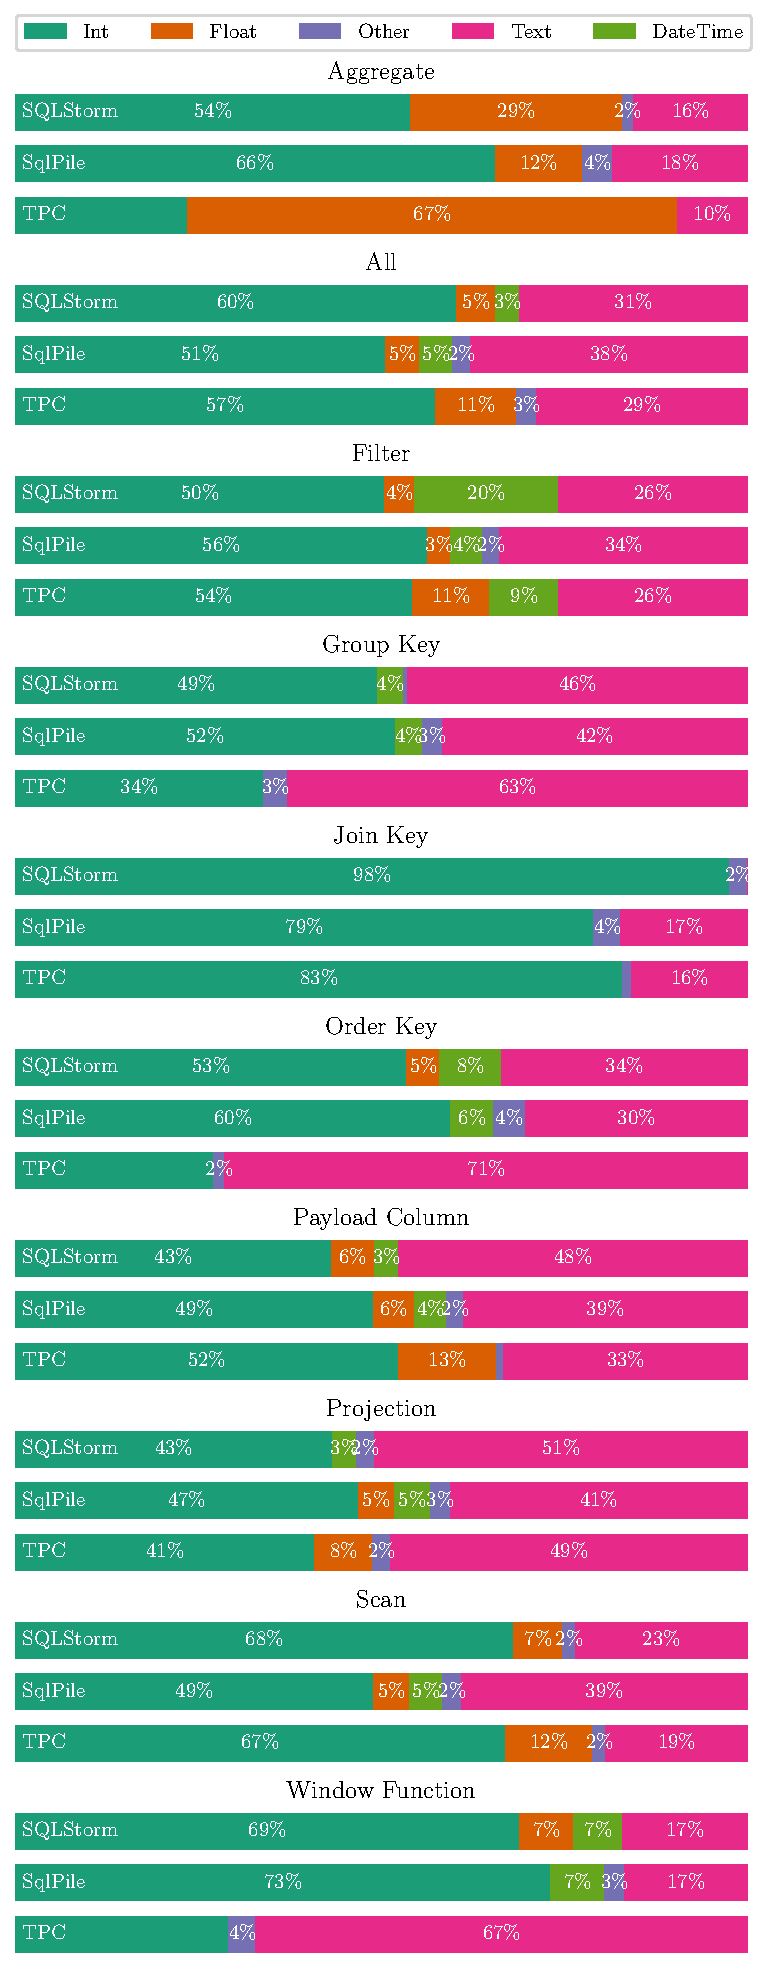
\includegraphics[width=\linewidth]{assets/column_usage/physical_type/column_cnt.pdf}
  \caption{Distribution of physical column types in SqlPile.}
  \Description{Distribution of physical column types in SqlPile.}
    \label{fig:column-physical-type-usage}
\end{figure}


\subsection{Semantic Type Analysis}\label{subsec:semantic-type-analysis}

In the following, we will discuss how which semantic type is used in which operator for different benchmarks (TPC-H, TPC-DS, SQLStorm).

\begin{figure}
  \centering
  
\includegraphics[width=\linewidth]{assets/column_usage/semantic_type_llm/column_cnt.pdf}
  \caption{Distribution of the semantic types of different benchmarks.}
  \Description{Distribution of the semantic types of different benchmarks.}
    \label{fig:column_semantic_type_usage}
\end{figure}

\begin{itemize}
\item Describe which semantic type is used in which operator. Go through operator by operator.
\item Highlight the differences between the different benchmarks (TPC-H, TPC-DS, SQLStorm)
\item Mention that boolean and numeric are merged to other types. 
\item Create a table with examples of the semantic type and how often it occured. Maybe add like a 2nd level of detail, e.g., for location: city, country, address, ...
\item What type of expressions are used for which operator and semantic type? 
\item What is the difference between the expressions in the different benchmarks?
\end{itemize}


\section{Benchmark for String}\label{sec:benchmark-for-string}
\begin{itemize}
    \item  Based on the analysis, we created a benchmark for strings.
    \item  What columns compress how well with which compression algorithm?
    \item  What are the expensive parts for e.g. a join operation of a int64 compared to a string?
    \item The goal should be to have a benchmark where both the compression and the execution can be tested.
    So the data is allowed to be compressed by the DBMS, the idea is to leverage how the data is compressed for execution.
    -> String processing is manly compressed execution
    \item The benchmark should measure compression speed, compression ratio, and execution speed, a bit similar then
    Clickbench but not with obscure queries then can be easily exploited on.
\end{itemize}

The idea for creating the benchmark is to get kaggle datasets (mainly ml datasets). They are usually denomalized single
tables so we could LLMs to normalize the data a bit more. Then we could use LLMs to generate very simple queries with
not that many joins. The benchmark should not be winable by good join ordering, but really focus on core operator
speed and the leverage of compression.
The problem of SQLstorm for string execution lays in the complexity of the queries. This means that good
query optimization will overshadow the actual execution performance.
Also, with only two new datasets, while there are a lot of different query features, there is a lack of divere data
features (Join on emails instead of uint64 ids, \ldots).

What do strings mean for GPU databases? Even more memory heavy..


\section{Findings}\label{sec:findings}
While the TPC-H schema defines a \texttt{comment} column for all tables
(e.g., \texttt{l\_comment}, \texttt{o\_comment}), only \texttt{c\_comment},
\texttt{o\_comment}, and \texttt{s\_comment} are actually used
This is especially noteworthy as also the comments from high cardinality tables like \texttt{lineitem} are not used.

Similar for TPC-DS, we only two out of five comment columns are used (\texttt{item\_desc} and \texttt{reason\_desc}).


\section{Limitations}\label{sec:limitations}
\begin{itemize}
    \item SQLPile contains a lot of simple queries. Many queries come not from suffisticated industrial applications, but
    from small personal projects.
    \item We only have a limited number of queries with joins and aggregations.
    \item While SQLPile contains mainly OLTP queries and schemas, kaggle are OLAP/ML datasets. We assume the properties of strings with
    the same semantic type are similar in both workloads.
\end{itemize}


\section{Recommendations for future Research}\label{sec:recommendations-for-future-research}

\begin{itemize}
    \item Strings are a catch it all type. We should not treat them as a single type, but accept that with differnt
    semantics come different properties that need to be treated differently.
    \item It is worth to do this, as strings are a significant part of the data stored and processed in DBMS.
\end{itemize}


\section{Related Work}\label{sec:related-work}
